

We return to the application of association screenings for categorical variables, and put the results in the previous section to use.
In particular, we focus on the exact-approximate support recovery problem, and demonstrate the consequences of its phase transition (Theorem \ref{thm:chi-squared-exact-approx-boundary}) in genetic association studies.

In order to do so, we must first connect the concept of ``statistical signal size'' $\lambda$ with some key quantities in association tests.
While ``signal size'' likely sounds foreign to most practitioners, it is intimately linked with the concept of ``effect sizes'' --- or odds ratios --- in association studies, which are frequently estimated and reported in GWAS catalogs.
We characterize the relationship between the two quantities in the special, but fairly common case of association tests on 2-by-2 contingency tables in Section \ref{subsec:odds-and-power}.


\subsection{Odds ratios and statistical power}
\label{subsec:odds-and-power}

% Unlike in additive models where the parameter $\mu$ has the interpretation of signal-to-noise ratios, the meaning of the signal sizes $\lambda$ in chi-square model is perhaps not as transparent.

Consider a 2-by-2 multinomial distribution with marginal probabilities of phenotypes $(\phi_1, \phi_2)$ and genotypes $(\theta_1, \theta_2)$.
The \emph{probability} table (as opposed to the table of multinomial \emph{counts} in the introduction) is as follows.
\begin{center}
    \begin{tabular}{cccc}
    \hline
    & \multicolumn{2}{c}{Genotype} \\
    \cline{2-3}
    Probabilities & Variant 1 & Variant 2 & Total by phenotype \\
    \hline
    Cases & $\mu_{11}$ & $\mu_{12}$ & $\phi_1$ \\
    Controls & $\mu_{21}$ & $\mu_{22}$ & $\phi_2$ \\
    Total by genotype & $\theta_1$ & $\theta_2$ & 1 \\
    \hline
    \end{tabular}
\end{center}
The odds ratio (i.e., ``effect size'') is defined as the ratio of the phenotype frequencies between the two genotype variants,
\begin{equation} \label{eq:odds-ratio}
    \text{R} := \frac{\mu_{11}}{\mu_{21}}\Big/\frac{\mu_{12}}{\mu_{22}}
    = \frac{\mu_{11}\mu_{22}}{\mu_{12}\mu_{21}}.
\end{equation}
The multinomial distribution is fully parametrized by the trio $(\theta_1, \phi_1, R)$.
Odds ratios further away from 1 indicate greater contrasts between the probability of outcomes.
Independence between the genotypes and phenotyes would imply an odds ratio of one, and hence $\mu_{jk} = \phi_j\theta_k$, for all $j,k \in\{1,2\}$.

% When data are sampled from the multinomial distribution, the chi-square test defined in \eqref{eq:chisq-statistic} is asymptotically equivalent to tests including, e.g., the likelihood ratio test and Welch's t-test, both in terms of level and power \cite{ferguson2017course,gao2019upass}.
For a sequence of local alternatives $\mu^{(1)}, \mu^{(2)}, \ldots$, such that $\sqrt{n}(\mu^{(n)}_{jk} - \phi_j\theta_k)$ converges to a constant table $\delta = (\delta_{jk})$, the chi-square test statistics converge in distribution to the non-central chi-squared distribution with non-centrality parameter 
$\lambda = \sum_{j=1}^2 \sum_{k=1}^2 {\delta_{jk}^2}/{(\phi_j\theta_k)}$; see, e.g.,\cite{ferguson2017course}.
Hence, for large samples from a fixed distribution $(\mu_{ij})$, the statistic is well approximated by a $\chi^2_1(\lambda)$ distribution, where
\begin{equation} 
\lambda = n\sum_{j=1}^2 \sum_{k=1}^2 \frac{(\mu_{jk} - \phi_j\theta_k)^2}{\phi_j\theta_k}.
\end{equation}
%Since $\lambda$ is linear in the number of samples $n$, 
% Power of association tests at $\alpha$ level is approximately $\P[\chi^2_{\nu}(\lambda)>\chi^2_{\nu,\alpha}]$, where $\chi^2_{\nu,\alpha}$ is the upper $\alpha$-quantile of a central Chi-squared distribution.
Power calculations therefore only depend on the $\mu_{jk}$'s through $\lambda=nw^2$, where we define 
\begin{equation} \label{eq:signal-size-chisq}
    w^2:=\lambda/n
\end{equation} 
to be the \emph{signal size per sample}. 
Statistical power would be increasing in $w^2$ for fixed sample sizes.

The next proposition states that the statistical signal size per sample can be parametrized by the odds ratio and the marginals in the probability table.

\begin{proposition} \label{prop:signal-size-odds-ratio}
Consider a 2-by-2 multinomial distribution with marginal distributions $(\phi_1, \phi_2 = 1-\phi_2)$ and $(\theta_1, \theta_2=1-\theta_1)$.
Let signal size $w^2$ be defined as in \eqref{eq:signal-size-chisq}, and odds ratio $\text{R}$ be defined as in \eqref{eq:odds-ratio}. 
If $R=1$, we have $w^2 = 0$; if $R\in(0,1)\cup(1,+\infty)$, then we have
\begin{equation} \label{eq:signal-size-odds-ratio}
    w^2(\text{R}) =
    \frac{1}{4A(\text{R}-1)^2}\left(B+CR-\sqrt{(B+CR)^2-4A(R-1)^2}\right)^2,
\end{equation}
where $A = \phi_1\theta_1\phi_2\theta_2$, $B = \phi_1\theta_1+\phi_2\theta_2$, and $C = \phi_1\theta_2+\phi_2\theta_1$.
\end{proposition}

Proposition \ref{prop:signal-size-odds-ratio} is derived in Appendix \ref{subsec:proof-signal-size-odds-ratio}. 

To understand Proposition \ref{prop:signal-size-odds-ratio}, we illustrate Relation \eqref{eq:signal-size-odds-ratio} for selected values of marginals $\theta_1$ and $\phi_1$ in Figure \ref{fig:signal-vs-odds}.
Observe in the figure that an odds ratio further away from one corresponds to stronger statistical signal per sample, ceteris paribus.
However, this ``valley'' pattern is in general not symmetric around 1, except for balanced marginal distributions ($\phi_1=1/2$ or $\theta_1=1/2$).
While the odds ratio $R$ can be arbitrarily close to 0 or diverge to $+\infty$ for any marginal distribution, the signal sizes $w^2$ are bounded from above by constants that depend only on the marginals.
% This is quantified in the next corollary.

\begin{figure}
      \centering
      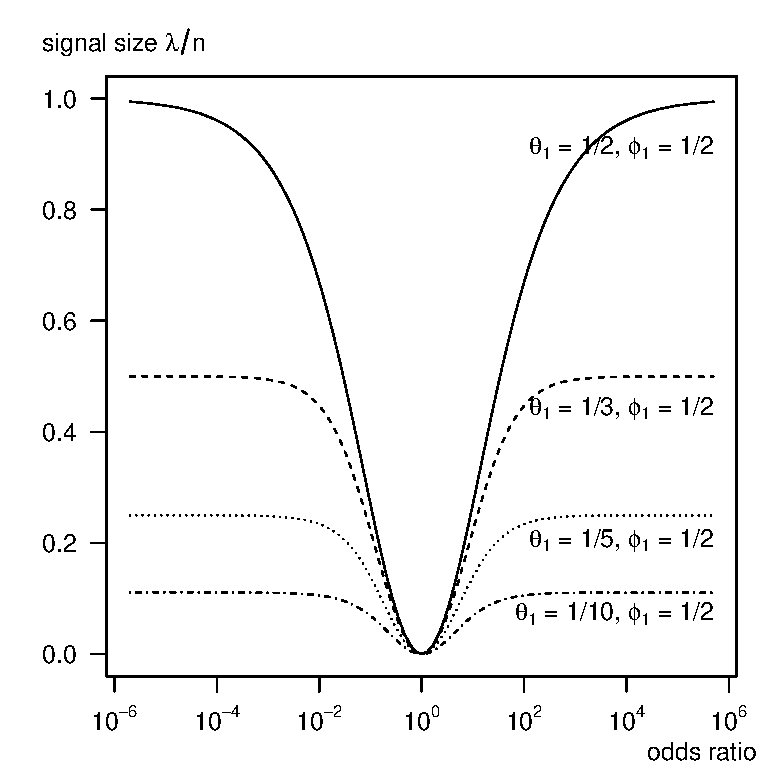
\includegraphics[width=0.49\textwidth]{./singal-vs-odds-p05}
      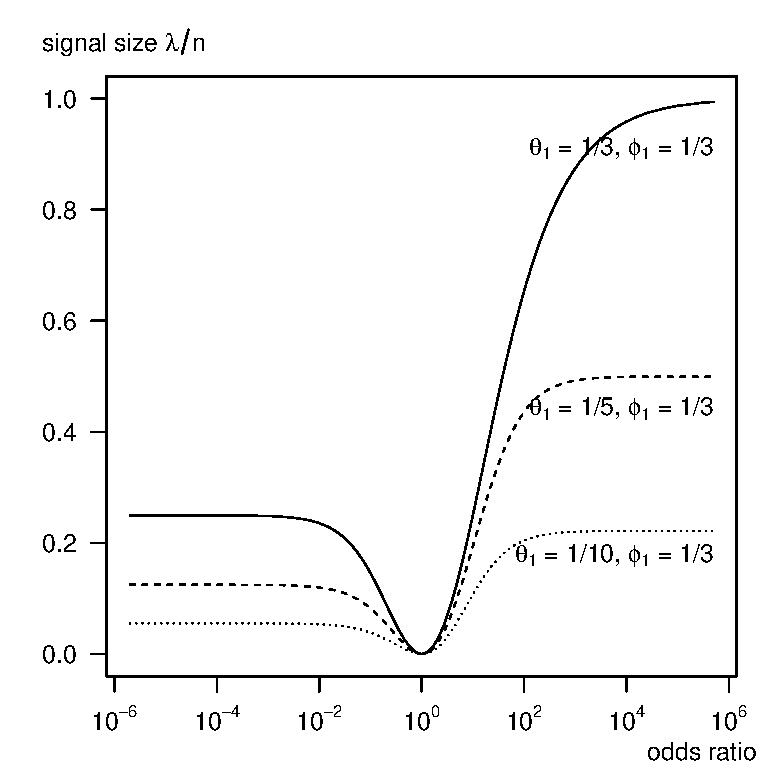
\includegraphics[width=0.49\textwidth]{./singal-vs-odds-p0333}            
      % 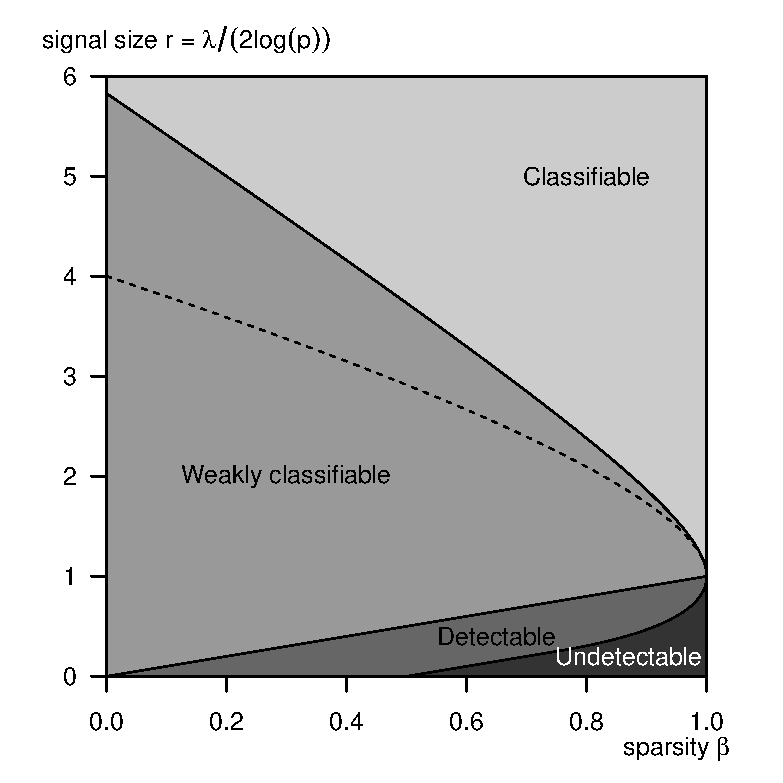
\includegraphics[width=0.35\textwidth]{./phase_diagram_chisquared.eps}
      \caption{Signal sizes per sample $w^2$ as functions of odds ratios in 2-by-2 multinomial distributions for selected genotype marginals in balanced (left) and unbalanced (right) designs; see Relation \eqref{eq:signal-size-odds-ratio} in Proposition \ref{prop:signal-size-odds-ratio}.
      For given marginal distributions, extreme odds ratios imply stronger statistical signals at a given sample size.
      However, the signal sizes are bounded above by constants that depend on the marginal distributions; see Relations \eqref{eq:signal-size-upper-bound-1} and \eqref{eq:signal-size-upper-bound-2}.
      % Unbalanced marginal distributions -- or rare variants -- lead to smaller signal sizes at a given odds ratio.
      } 
      \label{fig:signal-vs-odds}
\end{figure}

\begin{corollary} \label{cor:signal-limits-OR}
The signal size as a function of the odds ratio $w^2(R)$ is decreasing on $(0,1)$ and increasing on $(1,\infty)$, with limits
\begin{equation} \label{eq:signal-size-upper-bound-1}
    \lim_{\text{R}\to0_+} w^2(\text{R}) = \min\left\{\frac{\phi_1\theta_1}{\phi_2\theta_2}, \frac{\phi_2\theta_2}{\phi_1\theta_1}\right\},
\end{equation}
and
\begin{equation} \label{eq:signal-size-upper-bound-2}
    \lim_{\text{R}\to+\infty} w^2(\text{R}) = \min\left\{\frac{\phi_1\theta_2}{\phi_2\theta_1}, \frac{\phi_2\theta_1}{\phi_1\theta_2}\right\}.
\end{equation}
\end{corollary}
% Proof of Corollary \ref{cor:signal-limits-OR} is found in Appendix \ref{subsec:proof-signal-size-odds-ratio}. 

Corollary \ref{cor:signal-limits-OR} immediately implies that balanced designs with roughly equal number of cases and controls are not necessarily the most informative.

For example, in a study where a third of the recruited subjects carry the genetic variant positively correlated with the trait (i.e., $\theta_1=1/3$), an unbalanced design with $\phi_1=1/3$ would maximize $w^2$ at large odds ratios.
This unbalanced design is much more efficient compared to, say, a balanced design with $\phi_1=1/2$.
In the first case, we have $w^2\to1$ as $R\to\infty$; whereas in the second design, $w^2<1/2$ no matter how large $R$ is.
This difference can also be read by comparing the dashed curve ($\theta_1=1/3$, $\phi_1=1/2$) in the left panel of Figure \ref{fig:signal-vs-odds}, with the solid curve ($\theta_1=1/3$, $\phi_1=1/3$) in the right panel of Figure \ref{fig:signal-vs-odds}.

\subsection{Optimal study designs and rare variants}
\label{subsec:optimal-design} 

For a study with a fixed budget, i.e., a fixed total number of subjects $n$, the researcher is free to choose the fraction of cases $\phi_1$ to be included in the study.
A natural question is how this budget should be allocated to maximize the statistical power of discovery, or equivalently, the signal sizes $\lambda=nw^2$.

In principal, Relation \eqref{eq:signal-size-odds-ratio} can be optimized with respect to the fraction of cases $\phi_1$ in order to find optimal designs, if $\theta_1$ is known and held constant.
In practice, this is not the case.
While the fraction of cases can be controlled, the distributions of genotypes \emph{in the study} are often unknown prior to data collection, and can change with the case-to-control ratio.

Fortunately, the conditional distributions of genotypes in the healthy control groups are often estimated by existing studies, and are made available by consortiums such as the NHGRI-EBI GWAS catalog \cite{macarthur2016new}.
% Assume (after appropriate relabelling, hence without loss of generality) that the first variant is associated with an increased risk of disease, and is henceforth referred to as the risk variant.
We denote the conditional frequency of the first genetic variant in the control group as $(f, 1-f)$, where
$$
f := \mu_{21} / \phi_2.
$$
The multinomial probability is fully parametrized by the new trio: $(f, \phi_1, R)$.
\begin{center}
    \begin{tabular}{cccc}
    \hline
    & \multicolumn{2}{c}{Genotype} \\
    \cline{2-3}
    Probabilities & Variant 1 & Variant 2 & Total by phenotype \\
    \hline
    Cases & $\frac{\phi_1fR}{fR+1-f}$ & $\frac{\phi_1(1-f)}{fR+1-f}$ & $\phi_1$ \\
    Controls & $f(1-\phi_1)$ & $(1-f)(1-\phi_1)$ & $1-\phi_1$ \\
    \hline
    \end{tabular}
\end{center}
Proposition \ref{prop:signal-size-odds-ratio} may also be re-stated in terms of the new parametrization.

% Note that all these quantities refer to what is in the study, and differ from their counterparts in the general population.

\begin{corollary} \label{cor:signal-size-odds-ratio-conditional-frequency}
In the 2-by-2 multinomial distribution with marginals $(\phi_1, \phi_2 = 1-\phi_1)$, and conditional distribution of the variants in the control group $(f, 1-f)$,
Relation \eqref{eq:signal-size-odds-ratio} holds with $\theta_1 = {\phi_1fR}/{(fR+1-f)} + f(1-\phi_1)$ and $\theta_2 = 1-\theta_1$.
\end{corollary} 

The choice of $\phi_1$ now has a practical solution.

\begin{corollary} \label{cor:optimal-design}
In the context of Corollary \ref{cor:signal-size-odds-ratio-conditional-frequency},
the optimal design $(\phi^*_1, \phi^*_2)$ that maximizes the signal size per sample $w^2$ is prescribed by
\begin{equation} \label{eq:optimal-design}
    \phi_1^* = \frac{fR+1-f}{fR+1-f+\sqrt{R}}, \quad\text{and}\quad 
    \phi_2^* = 1-\phi_1^*.
\end{equation}
% when the denominator in \eqref{eq:optimal-design} is non-zero; otherwise, $\phi_1^*=\phi_2^*=1/2$.
\end{corollary} 

Proof of Corollary \ref{cor:optimal-design} is found in Appendix \ref{subsec:proof-signal-size-odds-ratio}. 

Of particular interest in the genetics literature are genetic variants with very low allele frequencies in the control group (i.e., $f\approx 0$), known as rare variants.
In such cases, Equation \eqref{eq:optimal-design} can be approximated using the Taylor expansion,
\begin{equation} \label{eq:optimal-design-approx}
    \phi_1^* = \frac{1}{1 + \sqrt{R}} + \frac{(R-\sqrt{R})f}{1+\sqrt{R}} + O(f^2).
\end{equation}
To illustrate, for rare and adversarial factors ($f\approx0$ and $R>1$), the optimal $\phi_1^*$ is less than $1/2$.
Therefore, for studies under a fixed budget, controls should constitute the majority of the subjects, in order to maximize power.
On the other hand, for rare and protective factors ($f\approx0$ and $R<1$), the optimal $\phi_1^*$ is greater than $1/2$, and cases should be the majority.

\subsection{Phase transitions in large-scale association screening studies}

% Specifically, we develop recipes to find suitable designs of association studies such that combination of the dimensionality $p$, sparsity $\beta$, and signal sizes $r$ of the problem lands in the desired region of risk control, as predicted by the results in Section \ref{sec:chisq-boundaries}.

% Of course, in applications, not all three of the parameters $(p, \beta, r)$ can be altered as we wish.
% In particular, the problem dimensions and sparsity levels are usually determined by the underlying physical processes.
% In the GWAS example, the number of genomic marker locations is determined by the chip used for gene sequencing, while the number of relevant genomic locations is a consequence of the biological process.
% Therefore, in order to achieve a desired level of error control, we can often only hope to influence the statistical signal sizes.

Returning to the problem of \emph{high-dimensional} marginal screenings for categorical covariates, we explore the manifestation of the phase transition in the exact-approximate support recovery problem in the genetic context.

Recall Theorem \ref{thm:chi-squared-exact-approx-boundary} predicts that FWER and FNR can be simultaneously controlled in large dimensions if and only if 
\begin{equation}
    r = \frac{\lambda}{2\log{p}} = \frac{w^2n}{2\log{p}} > 1.
\end{equation}
Therefore, if we were to apply FWER-controlling procedures at low nominal levels (say, $5\%$), then the FNR would experience a phase transition in the sense that, if
\begin{equation} \label{eq:power-1-region}
    r>1 \iff w^2 > \frac{2\log{p}}{n},
\end{equation}
then the FNR can be close to 0; otherwise, FNR must be close to 1.

% Translating this result into the language of association tests, 
Using the parametric relationship described in Corollary \ref{cor:signal-size-odds-ratio-conditional-frequency} (and Proposition \ref{prop:signal-size-odds-ratio}), 
the inequalities in \eqref{eq:power-1-region} implicitly define regions of $(f, R)$ where associations are discoverable with high power, for a given $\phi_1$.
Further, the boundary of such discoverable regions sharpens as dimensionality diverges. 
We illustrate this phase transition through a numerical example next.

\begin{figure}
      \centering
      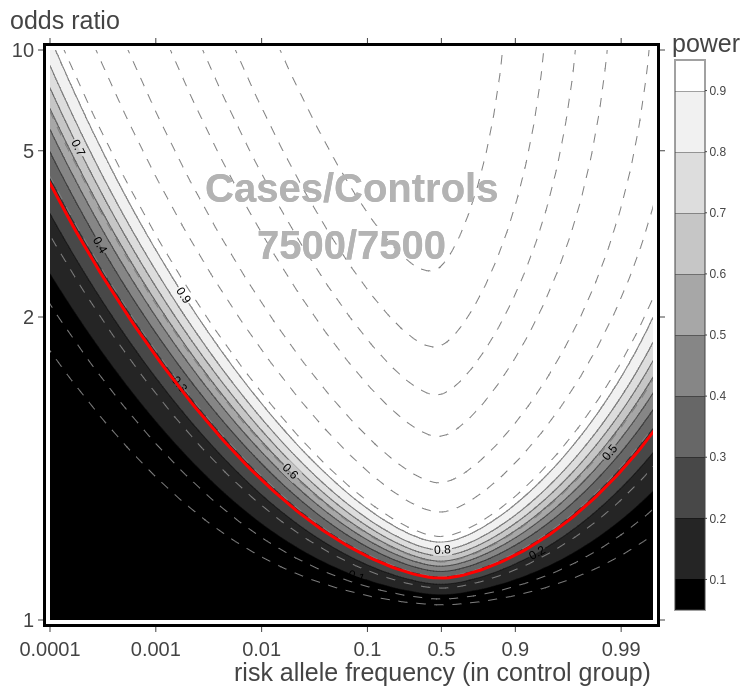
\includegraphics[width=0.49\textwidth]{./OR-RAF_plots/OR-RAF_p4.png} 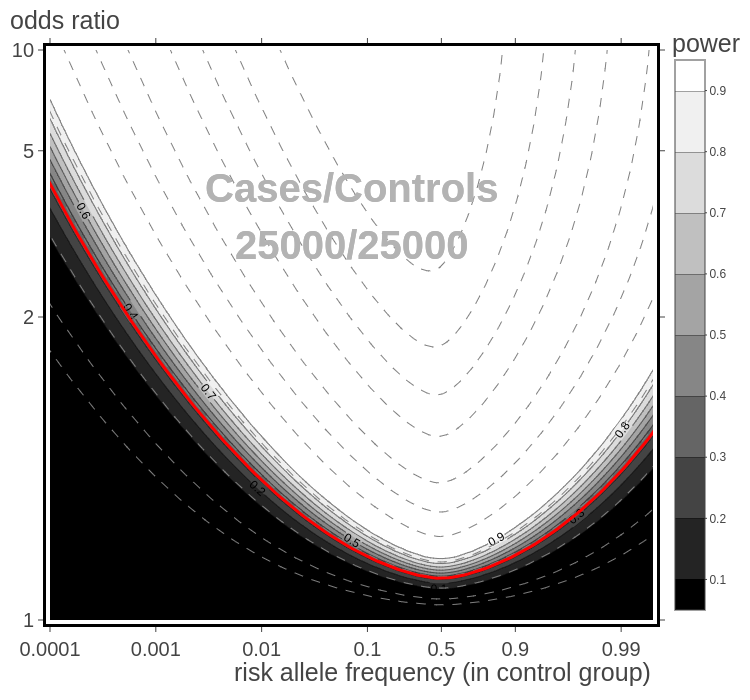
\includegraphics[width=0.49\textwidth]{./OR-RAF_plots/OR-RAF_p1e2.png} 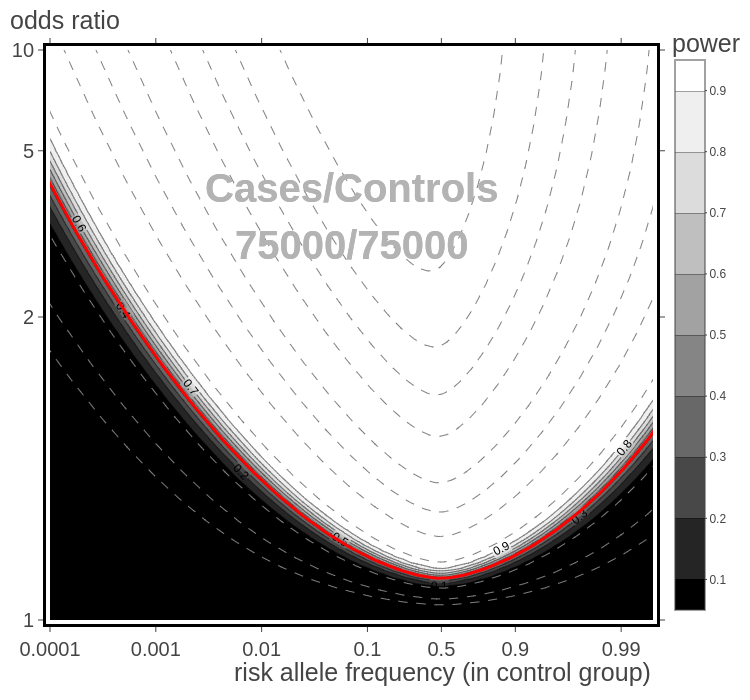
\includegraphics[width=0.49\textwidth]{./OR-RAF_plots/OR-RAF_p1e6.png} 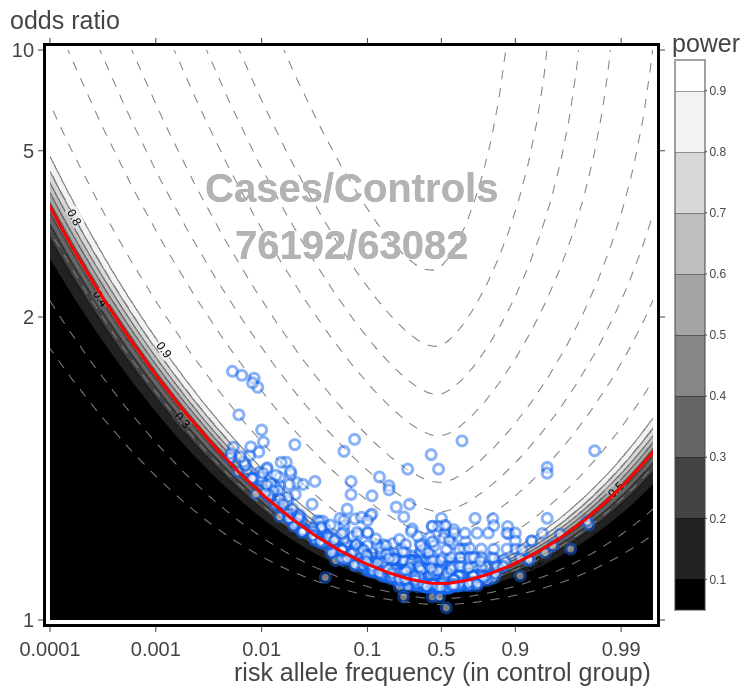
\includegraphics[width=0.49\textwidth]{./OR-RAF_plots/OR-RAF_BC_study.png}
      \caption{The OR-RAF diagram visualizing the marginal power of discovery in genetic association studies, after applying Bonferroni's procedure with nominal FWER at $5\%$ level. 
      Sample sizes are marked in each panel, and the problem dimensions are, respectively, $p=4$ (upper-left), $p=10^2$ (upper-right), and $p=10^6$ (lower-left), so that $n/\log{p}$ are roughly constant.
      Red curves mark the boundaries ($r=1$) of the phase transition for the exact-approximate support recovery problem; dashed curves are the equi-signal (equi-power) curves.
      The phase-transition in signal sizes $\lambda$ translates into the phase transition in terms of $(f,R)$, and sharpens as $p\to\infty$; see Example \ref{exmp:OR-RAF_phase_transition}.
      In the lower-right panel, we visualize discovered associations (blue circles) in a recent GWA study \cite{michailidou2017association}; the estimated odds ratios and risk allele frequencies are subject to survival bias and should not be taken at their face values; see Remark \ref{rmk:OR-RAF_false_evidence}.} 
      \label{fig:OR-RAF_GWAS}
\end{figure}


\begin{example}
\label{exmp:OR-RAF_phase_transition}
Consider association tests on $2\times2$ contingency tables at $p$ locations as introduced in Section \ref{subsec:motivation-chisq}, where the counts follow 
a multinomial distribution
% independent binomial distributions 
% $$
% O_{11} \sim \mathrm{Binom}(n\phi_1, fR/(fR+1-f)),\quad 
% O_{21} \sim \mathrm{Binom}(n(1-\phi_1), fR/(fR+1-f)),
% $$
parametrized by $(f, R, \phi_1)$ as in Section \ref{subsec:optimal-design}.
Assume that the phenotype marginals are fixed at $\phi_1 = \phi_2 = 1/2$.
% --- as is the case in genetic association studies --- 
Applying Bonferroni's procedure with nominal FWER at $\alpha=5\%$ level, we can approximate the marginal power of association tests by
\begin{equation} \label{eq:power-approximation}
    \P[\chi^2_{1}(\lambda)>\chi^2_{1,\alpha/p}],
\end{equation}
where $\chi^2_{1,\alpha/p}$ is the upper $(\alpha/p)$-quantile of a central chi-squared distribution with 1 degree of freedom.
We calculate this marginal power as a function of the parameters $(f,R)$ in three scenarios:
\begin{itemize}
    \item $p=4$, $n=3\times10^4$ 
    \item $p=10^2$, $n=1\times10^5$
    \item $p=10^6$, $n=3\times10^6$
\end{itemize}
and visualize the results as heatmaps\footnote{Since genetic variants can always be relabelled such that Variant 1 is positively associated with Cases, we only produce part of the diagram where $R>1$.
Sample sizes marked in the figure are adjusted by a factor of $1/2$, to reflect the genetic context where a pair of alleles are measured for every individual at every genomic location.} (referred to as OR-RAF diagrams) in Figure \ref{fig:OR-RAF_GWAS}.
These parameter values are chosen so that $\log{p}/n$ are roughly constant (around $4.6\times10^{-5}$).

We also overlay ``equi-signal'' curves, i.e., functions implicitly defined by the equations $r=c$ for a range of $c$ (dashed curves), and highlight the predicted boundary of phase transition for the exact-approximate support recovery problem $r=1$ (red curves).
The change in marginal power clearly sharpens around the predicted boundary $r=1$ as dimensionality diverges.
\end{example}

% --- or equivalently, the marginal power ---


\begin{remark}
\label{rmk:OR-RAF_false_evidence}
In an attempt to find empirical evidence of our theoretical predictions, we chart the genetic variants associated with breast cancer, discovered in a 2017 study by \citet{michailidou2017association} in an OR-RAF diagram. 
The estimated risk allele frequencies ($f$) and odds ratios ($R$) are taken from the NHGRI-EBI GWAS catalog \cite{macarthur2016new}, and plotted against a power heatmap calculated according to the reported sample sizes. 
See lower-right panel of Figure \ref{fig:OR-RAF_GWAS}.

It is tempting to believe, on careless inspection, that roughly \emph{all} discovered associations fall inside the high power region of the diagram, therefore demonstrating the phase transition in statistical power.
Unfortunately, the estimates here are subject to survival {bias} --- the study in fact uses the {same} dataset for \emph{both} support estimation and parameter estimation, without adjusting the latter for the selection process.
The seemingly striking agreement between the power calculations and the estimated effects of reported associations \emph{should not} be taken as evidence for the validity of our theory.
Nevertheless, we conjecture, as the theory predicts, that accurate and unbiased parameter estimates from an independent replication will still place the associations in the high power region of the diagram. 
\end{remark}

Finally, we demonstrate with an example how results in Sections \ref{sec:chisq-boundaries} and \ref{sec:signal-size-odds-ratio} may be used for planning prospective association studies.

\begin{example}
In a GWAS with $p = 10^6$ genomic marker locations, researchers wish to locate genetic associations with the trait of interest.
Specifically, they wish to maximize power in the region where genetic variants have risk allele frequencies of $0.01$ and odds ratios of $1.2$.
By Corollary \ref{cor:optimal-design}, the optimal design has a fraction of cases $\phi^* = 0.478$, yielding the statistical signal size per sample $w^2\approx9.00\times10^{-5}$ according to Corollary \ref{cor:signal-size-odds-ratio-conditional-frequency}.

If we wish to achieve exact-approximate support recovery in the sense of \eqref{eq:support-recovery-success}, Theorem \ref{thm:chi-squared-exact-approx-boundary} predicts that the signal size parameter $r$ has to be at least $\widetilde{g}(\beta)= 1$.
This signal size calls for a sample size of $n = \lambda / w^2 = 2r\log(p)/w^2 \approx 307,011$.
In a typically GWAS, a pair of alleles are sequenced for every marker location, bringing the required number of subjects in the study to $n/2 \approx 153,509$.
\end{example}

In comparison, a more accurate power calculation directly using \eqref{eq:power-approximation} predicts that $n / 2 = 165,035$ subjects are needed, under the set of parameters ($p=10^6$, $f=0.01$, $R=1.2$) and $\mathrm{FWER}=0.05$, $\mathrm{FNR}=0.5$; this is $7\%$ higher than our crude asymptotic approximation.
% The accuracy of the asymptotic approximations, by nature of the statements in Theorem \ref{thm:chi-squared-exact-boundary} and \ref{thm:chi-squared-approx-boundary}, depends on how close the error metrics are to zero.
% For example, the number of subjects needed for $\mathrm{FWER}=\mathrm{FWNR}=0.01$ is $499,598$, an $8\%$ increase over the asymptotic prediction; at $\mathrm{FWER}=\mathrm{FWNR}=0.1$, this number becomes $398,996$, some $14\%$ lower than the asymptotic result.
In general, we recommend using the more precise calculations over the back-of-the-envelope asymptotics for planning prospective studies and performing systematic reviews;
a user-friendly web application implementing the more precise approximations is provided in \cite{gao2019upass}.
Nevertheless, the phase transition results generate simple but powerful insights that cannot be easily supplanted.
